\documentclass{standalone}
\usepackage{tikz}
\usepackage{ctex,siunitx}
\setCJKmainfont{Noto Serif CJK SC}
\usepackage{tkz-euclide}
\usepackage{amsmath}
\usetikzlibrary{patterns, calc}
\usetikzlibrary {decorations.pathmorphing, decorations.pathreplacing, decorations.shapes,}
\begin{document}
\small
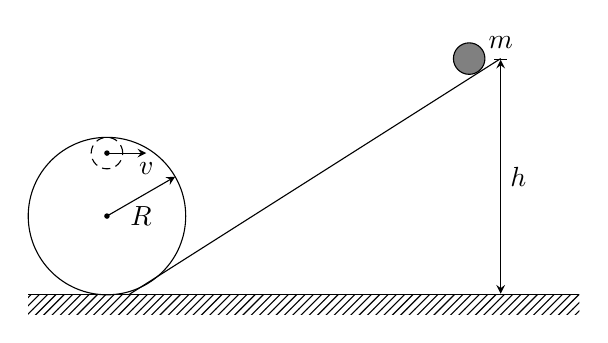
\begin{tikzpicture}[>=stealth,scale=1]
  \draw (-1,0)--(6,0);
  \fill [pattern = north east lines] (-1,-.25) rectangle (6,0);
  \draw (0,1) circle(1);
  \draw (.275,0)--(5,3);
  \draw [|<->|](5,0)--node [right]{$h$}(5,3)node[above]{$m$};
  \draw [fill=gray](4.6,3) circle (.2);
  \draw [densely dashed](0,2-.2) circle (.2);
  \draw[->](0,1)--node [below]{$R$}+(30:1);
  \draw [->](0,2-.2)--(.5,2-.2)node[below]{$v$};
  \fill (0,1) circle(1pt);
  \fill (0,2-.2) circle(1pt);
\end{tikzpicture}
\end{document}